\begin{spacing}{2}
    \section{实验}
\end{spacing}
\subsection{网络初始化设计}
使用Adam Optimizer,经过初步实验,学习率定为$1^{-5}$。卷积核使用Xavier初始化方法。实验共进行两组,具体参数如表\ref{Tab:test}所示。
\begin{table}[htbp]
    
    \centering
    \caption{实验分组}
    \label{Tab:test}
    \scalebox{1.0}{
        \begin{tabular}{cc}
            \toprule  %添加表格头部粗线
            组别   & 损失函数       \\
            \midrule  %添加表格中横线
            第一组 & 交叉熵         \\
            第二组 & 类别平衡交叉熵 \\
            \hline \hline
        \end{tabular}
    }
    
\end{table}
\subsection{实验结果}
每组实验都经过3000次左右迭代,训练时间约12小时。由于在训练过程中生成预测结果耗时巨大,因此只在测试训练阶段生成了预测结果。后面的典型错误一节的内容是在测试训练阶段生成的,并不是实际训练阶段的结果。
\subsubsection{第一组:交叉熵}

使用交叉熵作为损失函数的组别最开始的正确率为0.72左右,损失为0.68左右。经过3000轮的迭代,正确率达到0.84左右,损失稳定在0.42左右,可见图\ref{Fig:g1_f1}及图\ref{Fig:g1_f2}。

\begin{figure}[htbp]
    
    \centering
    \begin{minipage}[t]{0.49\textwidth}
        \centering
        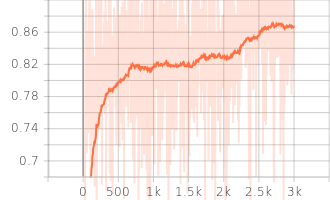
\includegraphics[width=1\textwidth]{Figures/图表/交叉熵/accuracy.png}
        \caption{第一组:准确率}
        \label{Fig:g1_f1}
    \end{minipage}
    \begin{minipage}[t]{0.49\textwidth}
        \centering
        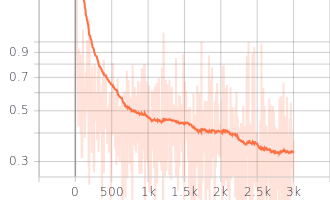
\includegraphics[width=1\textwidth]{Figures/图表/交叉熵/cost.png}
        \caption{第一组:损失}
        \label{Fig:g1_f2}
    \end{minipage}
    
\end{figure}

使用类别交叉熵作为损失函数的组别最开始的交叉熵为0.68左右,F1 Score为0.31左右,交叉熵为0.56左右。经过3000轮的迭代,交叉熵达到0.42左右,F1 Score稳定在0.47左右,可见图\ref{Fig:g1_f3}及图\ref{Fig:g1_f4}。

\begin{figure}[htbp]
    
    \centering
    \begin{minipage}[t]{0.49\textwidth}
        \centering
        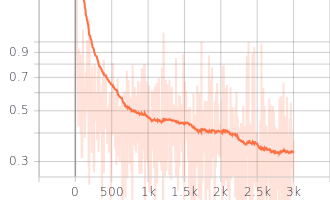
\includegraphics[width=1\textwidth]{Figures/图表/交叉熵/cross_entropy.png}
        \caption{第一组:交叉熵}
        \label{Fig:g1_f3}
    \end{minipage}
    \begin{minipage}[t]{0.49\textwidth}
        \centering
        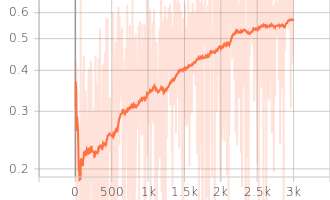
\includegraphics[width=1\textwidth]{Figures/图表/交叉熵/f1_score.png}
        \caption{第一组:F1 Score}
        \label{Fig:g1_f4}
    \end{minipage}
    
\end{figure}

使用类别交叉熵作为损失函数的组别最开始的精确率为0.18左右,召回率为0.44左右,交叉熵为0.56左右。经过3000轮的迭代,精确率达到0.60左右,召回率稳定在0.43左右,可见图\ref{Fig:g1_f5}及图\ref{Fig:g1_f6}。

\begin{figure}[htbp]
    
    \centering
    \begin{minipage}[t]{0.49\textwidth}
        \centering
        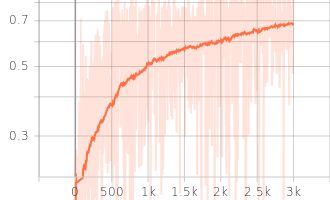
\includegraphics[width=1\textwidth]{Figures/图表/交叉熵/precision.png}
        \caption{第一组:精确率}
        \label{Fig:g1_f5}
    \end{minipage}
    \begin{minipage}[t]{0.49\textwidth}
        \centering
        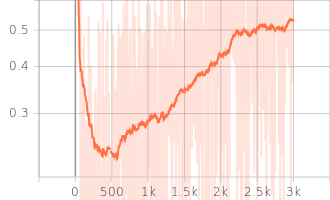
\includegraphics[width=1\textwidth]{Figures/图表/交叉熵/recall.png}
        \caption{第一组:召回率}
        \label{Fig:g1_f6}
    \end{minipage}
    
\end{figure}

\subsubsection{第二组:类别平衡交叉熵}

使用类别交叉熵作为损失函数的组别最开始的正确率为0.68左右,损失为0.32左右。经过3000轮的迭代,正确率达到0.83左右,损失稳定在0.27左右,可见图\ref{Fig:g2_f1}及图\ref{Fig:g2_f2}。

\begin{figure}[htbp]
    
    \centering
    \begin{minipage}[t]{0.49\textwidth}
        \centering
        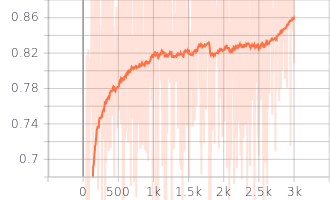
\includegraphics[width=1\textwidth]{Figures/图表/类别平衡交叉熵/accuracy.png}
        \caption{第二组:准确率}
        \label{Fig:g2_f1}
    \end{minipage}
    \begin{minipage}[t]{0.49\textwidth}
        \centering
        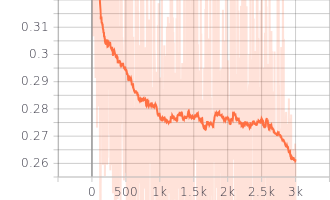
\includegraphics[width=1\textwidth]{Figures/图表/类别平衡交叉熵/cost.png}
        \caption{第二组:损失}
        \label{Fig:g2_f2}
    \end{minipage}
    
\end{figure}

使用类别交叉熵作为损失函数的组别最开始的交叉熵为0.57左右,F1 Score为0.46左右,交叉熵为0.56左右。经过3000轮的迭代,交叉熵达到0.40左右,F1 Score稳定在0.51左右,可见图\ref{Fig:g2_f3}及图\ref{Fig:g2_f4}。

\begin{figure}[htbp]
    
    \centering
    \begin{minipage}[t]{0.49\textwidth}
        \centering
        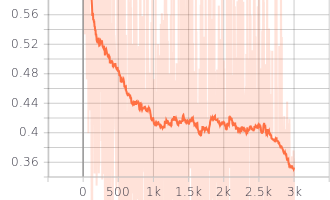
\includegraphics[width=1\textwidth]{Figures/图表/类别平衡交叉熵/cross_entropy.png}
        \caption{第二组:交叉熵}
        \label{Fig:g2_f3}
    \end{minipage}
    \begin{minipage}[t]{0.49\textwidth}
        \centering
        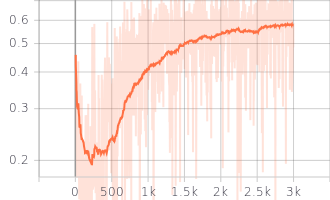
\includegraphics[width=1\textwidth]{Figures/图表/类别平衡交叉熵/f1_score.png}
        \caption{第二组:F1 Score}
        \label{Fig:g2_f4}
    \end{minipage}
    
\end{figure}

使用类别交叉熵作为损失函数的组别最开始的精确率为0.31左右,召回率为0.54左右,交叉熵为0.56左右。经过3000轮的迭代,精确率达到0.58左右,召回率稳定在0.5左右,可见图\ref{Fig:g2_f5}及图\ref{Fig:g2_f6}。

\begin{figure}[htbp]
    
    \centering
    \begin{minipage}[t]{0.49\textwidth}
        \centering
        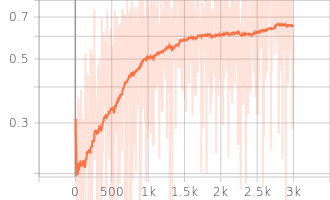
\includegraphics[width=1\textwidth]{Figures/图表/类别平衡交叉熵/precision.png}
        \caption{第二组:精确率}
        \label{Fig:g2_f5}
    \end{minipage}
    \begin{minipage}[t]{0.49\textwidth}
        \centering
        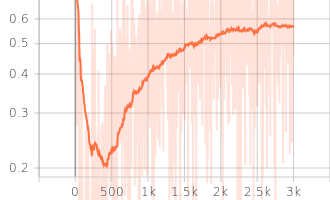
\includegraphics[width=1\textwidth]{Figures/图表/类别平衡交叉熵/recall.png}
        \caption{第二组:召回率}
        \label{Fig:g2_f6}
    \end{minipage}
    
\end{figure}
\subsubsection{结果分析}
\begin{table}[htbp]
    
    \centering
    \caption{试验结果}
    \label{Tab:result_compare}
    \scalebox{1.0}{
        \begin{tabular}{cccccc}
            \toprule  %添加表格头部粗线
            组别           & 正确率 & 交叉熵 & F1 Score & 精确率 & 召回率 \\
            \midrule  %添加表格中横线
            交叉熵         & 0.84   & 0.42   & 0.47     & 0.6    & 0.43   \\
            类别平衡交叉熵 & 0.83   & 0.40   & 0.51     & 0.58   & 0.50   \\
            \hline \hline
        \end{tabular}
    }
    
\end{table}
从结果上看,两种方法在正确率和交叉熵上没有太大差别,以交叉熵作为损失函数略优于以类别平衡交叉熵方法。但是这两种方法在F1 Score上有较大差别。交叉熵的F1 Score为0.47,类别平衡交叉熵的F1 Score为0.51,类别平衡交叉熵较交叉熵提高了8.5\%。下面对这一原因具体分析。

两种方法在精确率上差别不大,交叉熵是0.6,类别平衡交叉熵是0.58;但在召回率上差别较大,交叉熵为0.43类别平衡交叉熵为0.5。类别平衡交叉熵较交叉熵提高了16\%。精确率指的是预测中正确正类的数量占所有预测中正类数量的比值。在这一指标上,交叉熵稍稍优于类别平衡交叉熵。我们从交叉熵的正确率稍高于类别平衡交叉熵这一点上也可以发现。但是在召回率这项指标上,两种方法差别巨大。交叉熵为0.43类别平衡交叉熵为0.5,类别平衡交叉熵较交叉熵提高了16\%。召回率指的是预测正确的正类占样本正类的比值。也就是说,类别平衡交叉熵能更完整地找出图像中的房屋。我们从网络生成的预测图中也可以发现,交叉熵检测出的房屋较类别平衡交叉熵更为破碎,完整性没有类别平衡交叉熵好。而类别平衡交叉熵能更完整地检测出房屋。
\subsection{典型错误}
\subsubsection{建筑过大}

由于本次统一将图片裁成$256\times 256$大小,因此有些过大的建筑在整张图像中有所缺失。如图\ref{Fig:big_building},本应整张图片都被识别为建筑,但是由于该建筑的范围超过了$256\times256$,因此未能完全识别。
\begin{figure}[htbp]
    
    \centering
    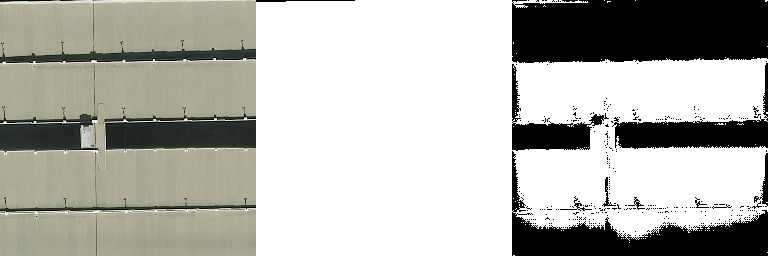
\includegraphics[width=1\textwidth]{Figures/错误/建筑过大.png}
    \caption{建筑过大}
    \label{Fig:big_building}
    
\end{figure}

同样的错误还出现在中等大小的建筑上,如图\ref{Fig:middle_building}。由于感受野大小不能包含整个建筑,所以建筑的中央未能正确识别为建筑。
\begin{figure}[htbp]
    
    \centering
    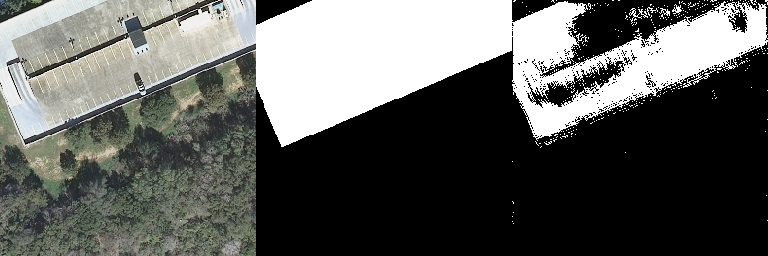
\includegraphics[width=1\textwidth]{Figures/错误/中等建筑.png}
    \caption{中等大小建筑错误}
    \label{Fig:middle_building}
    
\end{figure}

\subsubsection{错认}

另一类典型错误是将道路和汽车错认为房屋如图\ref{Fig:error_road}。由于道路和房屋的边缘比较相像,所以常有道路被错认为房屋的情况出现。
\begin{figure}[htbp]
    
    \centering
    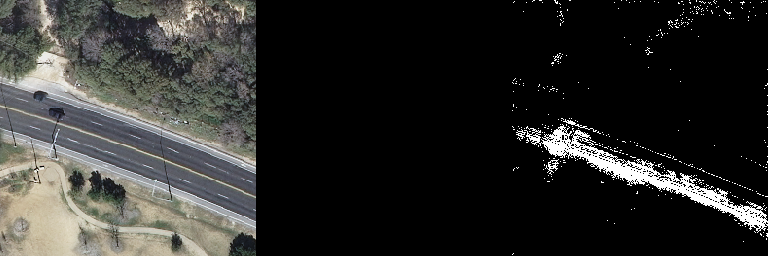
\includegraphics[width=1\textwidth]{Figures/错误/道路错认.png}
    \caption{道路错认}
    \label{Fig:error_road}
    
\end{figure}

另外,并排停放的汽车大小和形状与小型房屋相似,也经常被错认为房屋,如图\ref{Fig:error_car}。
\begin{figure}[htbp]
    
    \centering
    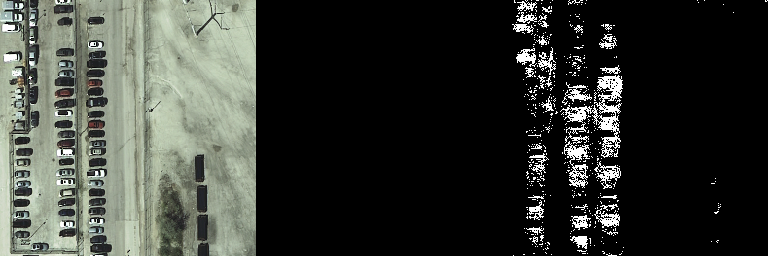
\includegraphics[width=1\textwidth]{Figures/错误/汽车错认.png}
    \caption{汽车错认}
    \label{Fig:error_car}
    
\end{figure}

\subsubsection{树木和光影}

树木遮挡是造成误差的另外一个主要原因,如图\ref{Fig:tree_error}。后期可能可以通过霍夫变换找到规则建筑的边界补齐。
\begin{figure}[htbp]
    
    \centering
    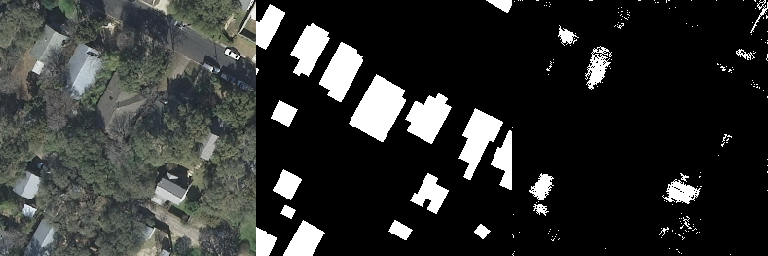
\includegraphics[width=1\textwidth]{Figures/错误/树木遮挡.png}
    \caption{树木遮挡}
    \label{Fig:tree_error}
    
\end{figure}

另外由于该图像集中建筑屋顶都较周围物体明亮,因此一些屋顶过暗的建筑可能不能被正确识别,如图\ref{Fig:dark_building}。
\begin{figure}[htbp]
    
    \centering
    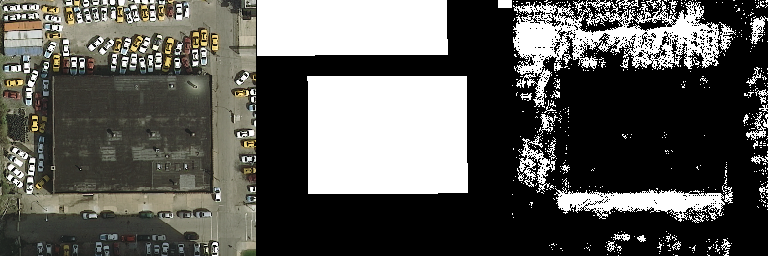
\includegraphics[width=1\textwidth]{Figures/错误/建筑过暗.png}
    \caption{建筑过暗}
    \label{Fig:dark_building}
    
\end{figure}

\subsection{最终结果}

由于该神经网络去掉了全连接层,使用全卷积层,因此该神经网络对输入图像的大小没有限制。我从测试数据集中选取了维也纳和奥斯汀地区的遥感图像作为测试。这两张遥感图像的大小为$5000\times 5000$像素,为了便于裁剪,我将其重新调整大小至$4096\times 4096$像素,然后切割成16张$1024\times 1024$的图像送入卷积神经网络进行计算。

图\ref{Fig:test_image_1}是维也纳地区的遥感图像;图\ref{Fig:test_image_1_gt}是该地区遥感图像的ground-truth。
\begin{figure}[htbp]
    
    \centering
    \begin{minipage}[t]{0.49\linewidth}
        \centering
        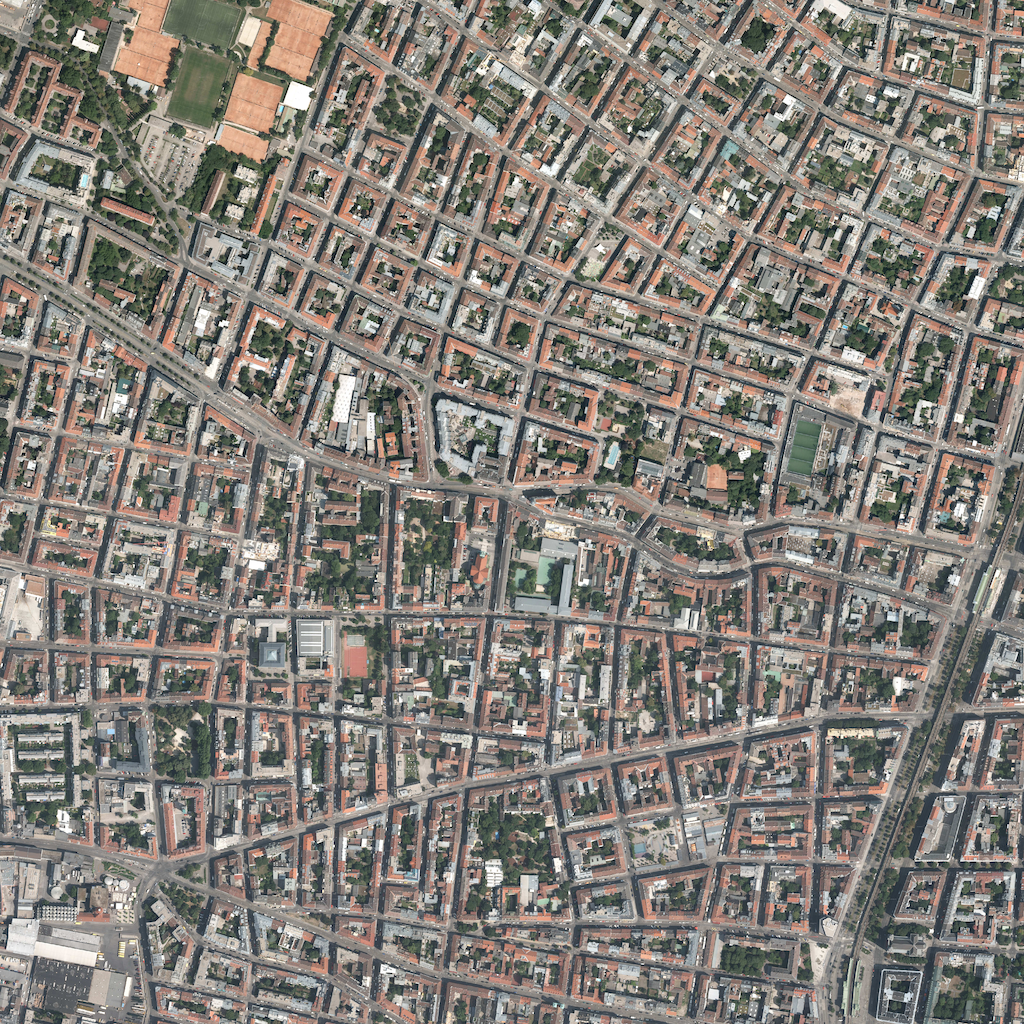
\includegraphics[width=1\linewidth]{Figures/结果/vienna8.png}
        \caption{维也纳}
        \label{Fig:test_image_1}
    \end{minipage}
    \begin{minipage}[t]{0.49\linewidth}
        \centering
        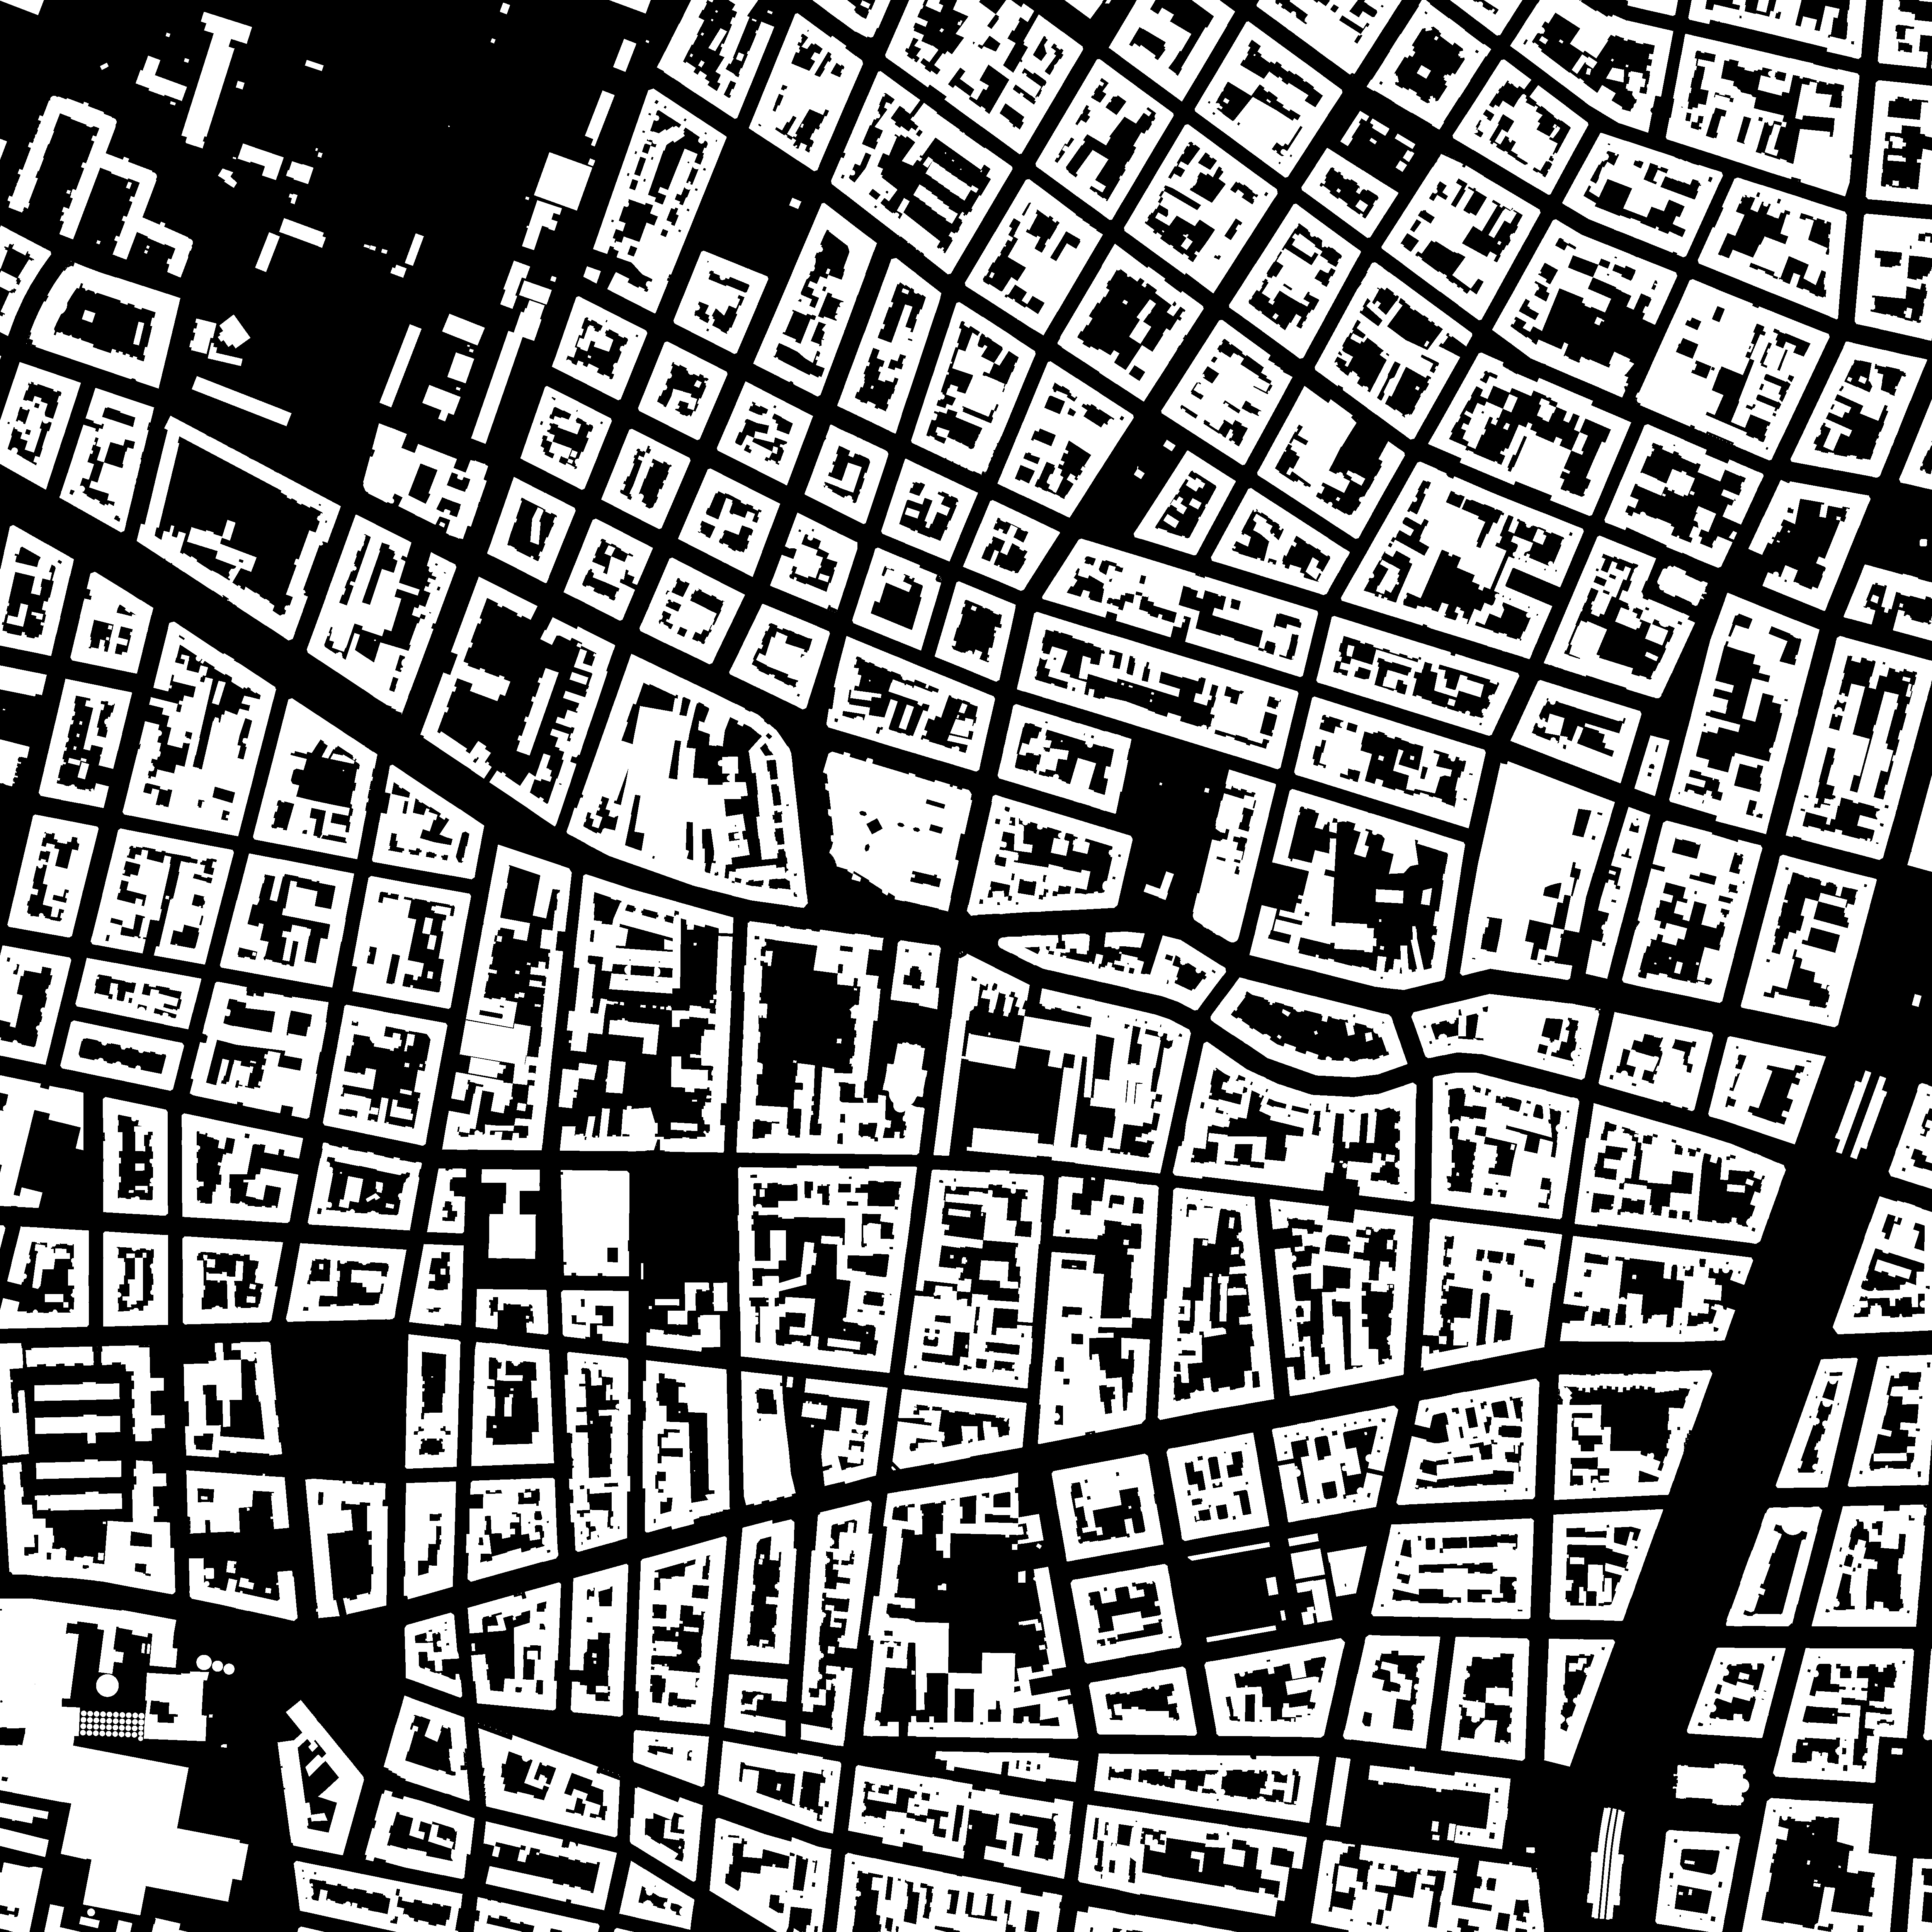
\includegraphics[width=1\linewidth]{Figures/结果/vienna8_gt.png}
        \caption{维也纳ground-truth}
        \label{Fig:test_image_1_gt}
    \end{minipage}
    
\end{figure}

图\ref{Fig:test_image_1_ce}是使用交叉熵作为损失函数的维也纳地区的预测结果;图\ref{Fig:test_image_1_cbce}是使用类别平衡交叉熵作为损失函数的维也纳地区的预测结果。
\begin{figure}[htbp]
    
    \centering
    \begin{minipage}[t]{0.49\linewidth}
        \centering
        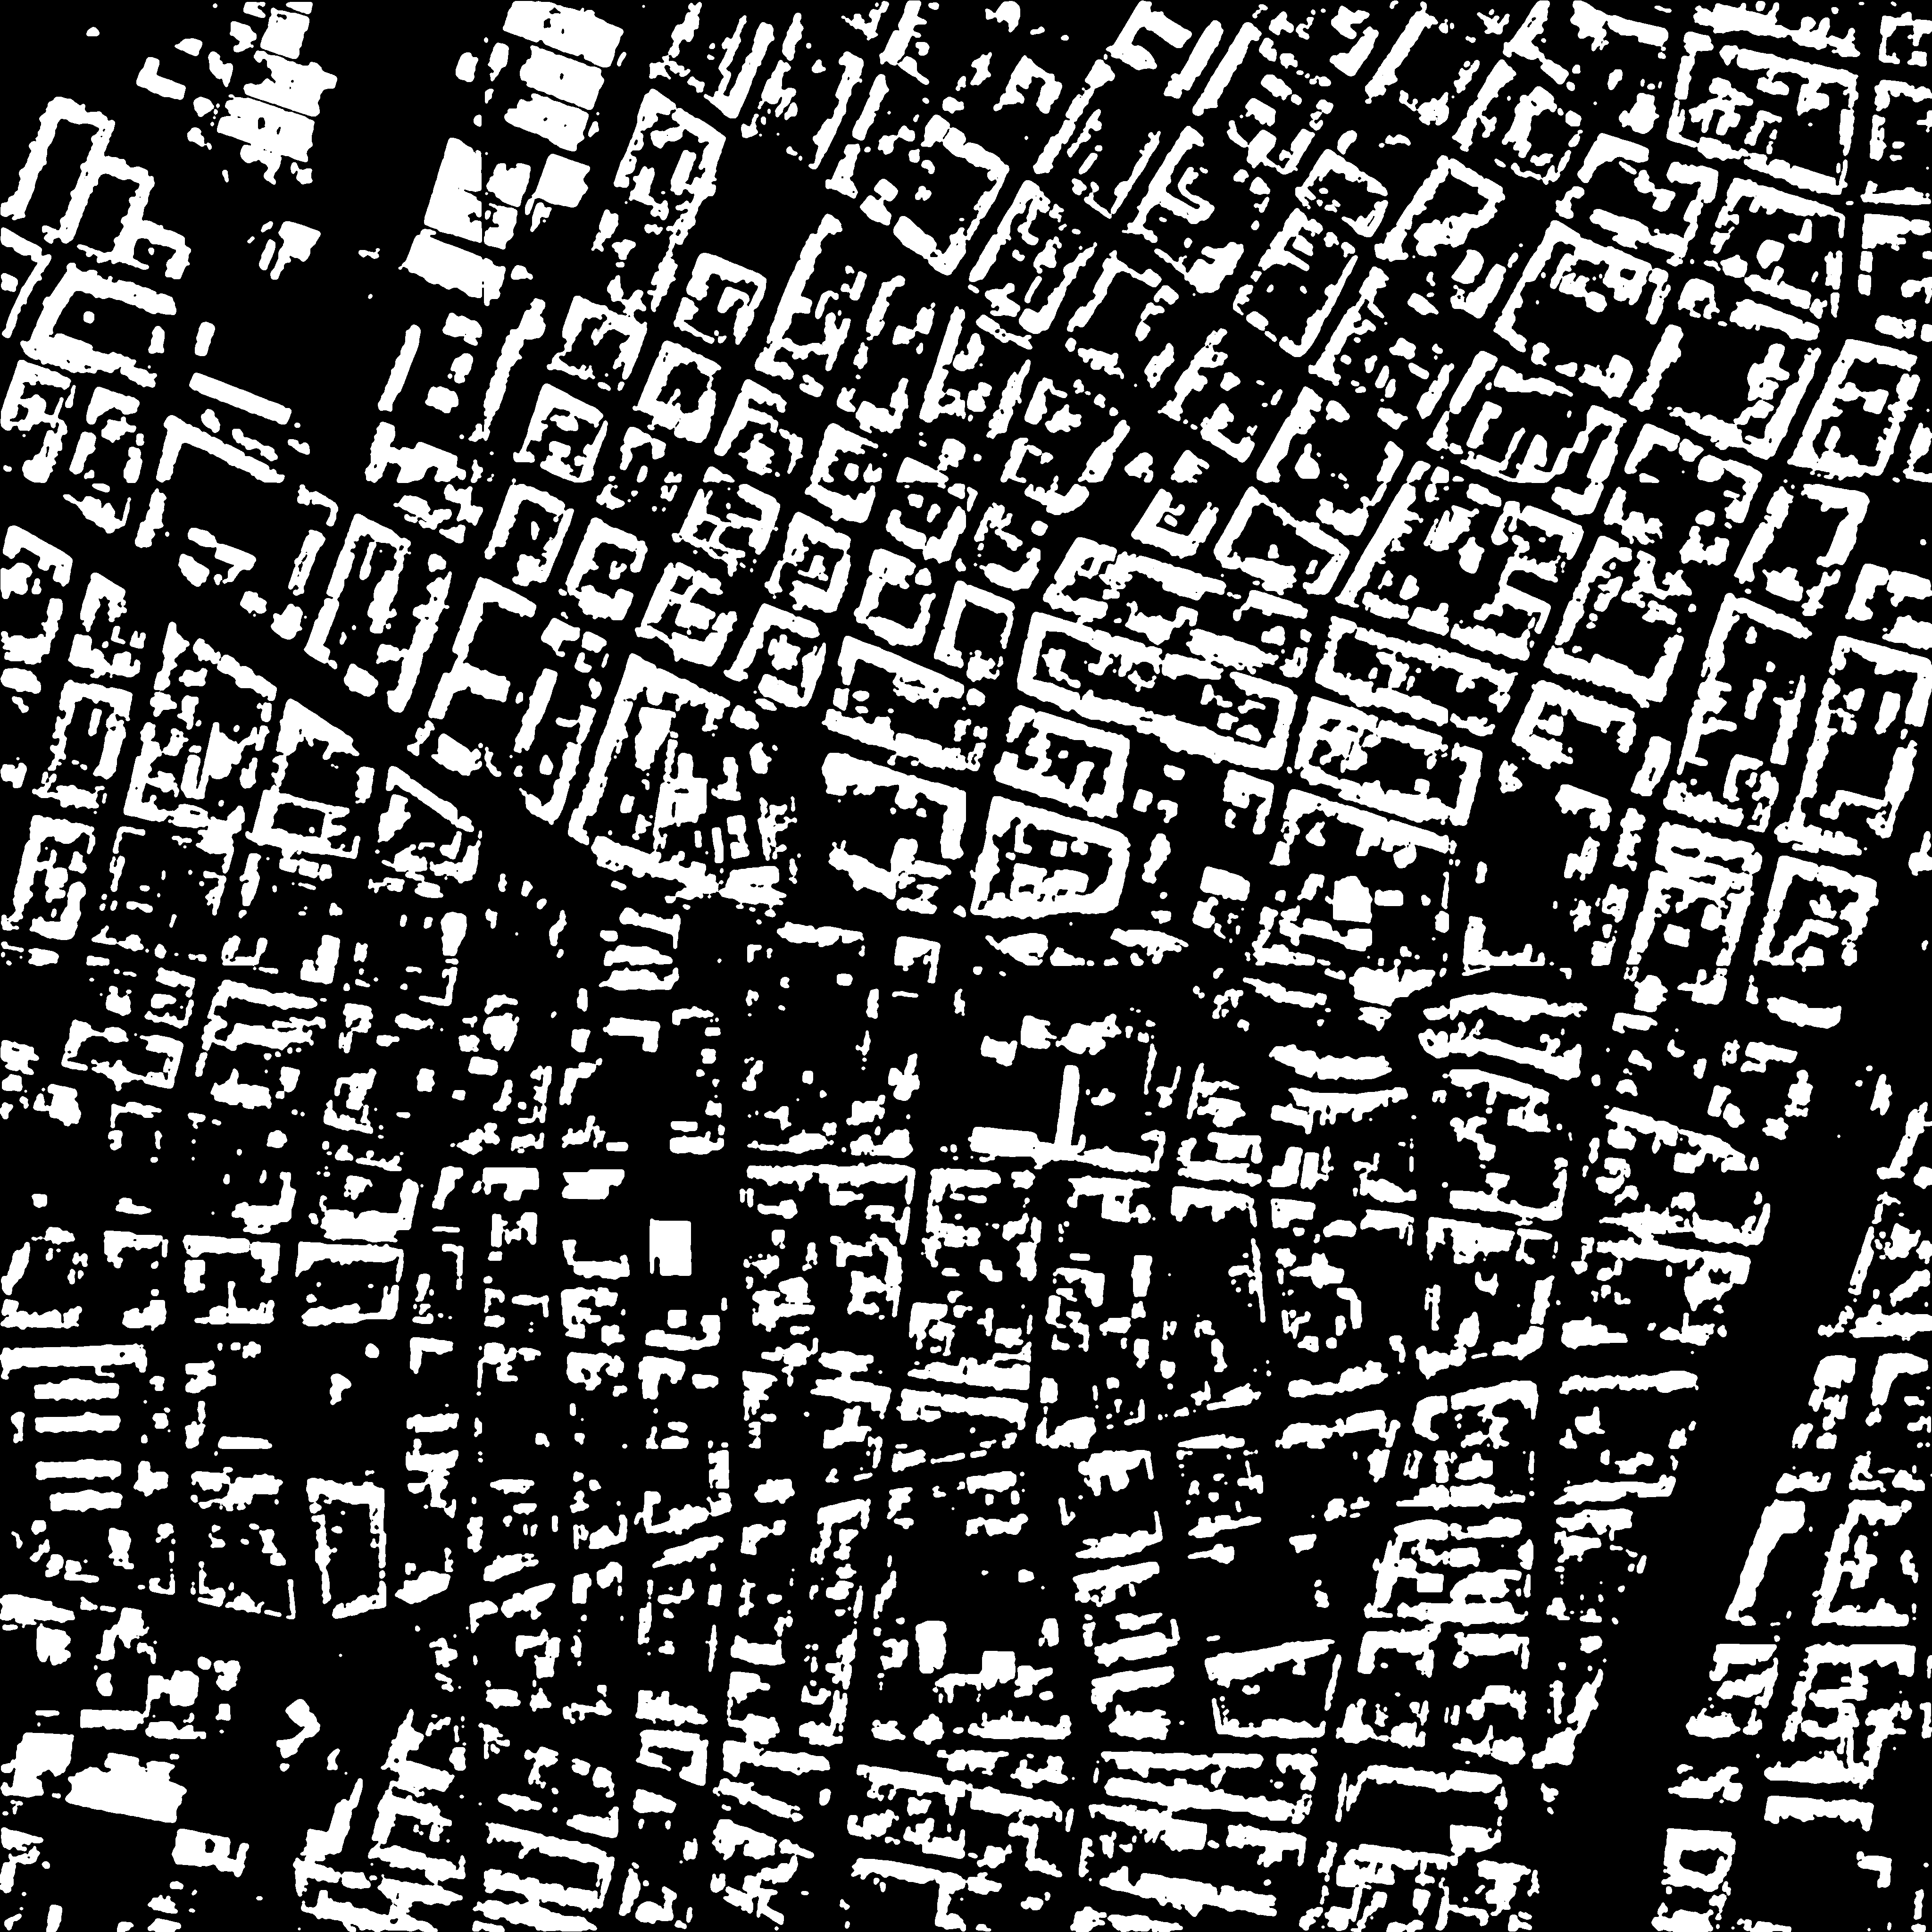
\includegraphics[width=1\linewidth]{Figures/结果/vienna8_交叉熵_中值滤波.png}
        \caption{维也纳—交叉熵}
        \label{Fig:test_image_2_ce}
    \end{minipage}
    \begin{minipage}[t]{0.49\linewidth}
        \centering
        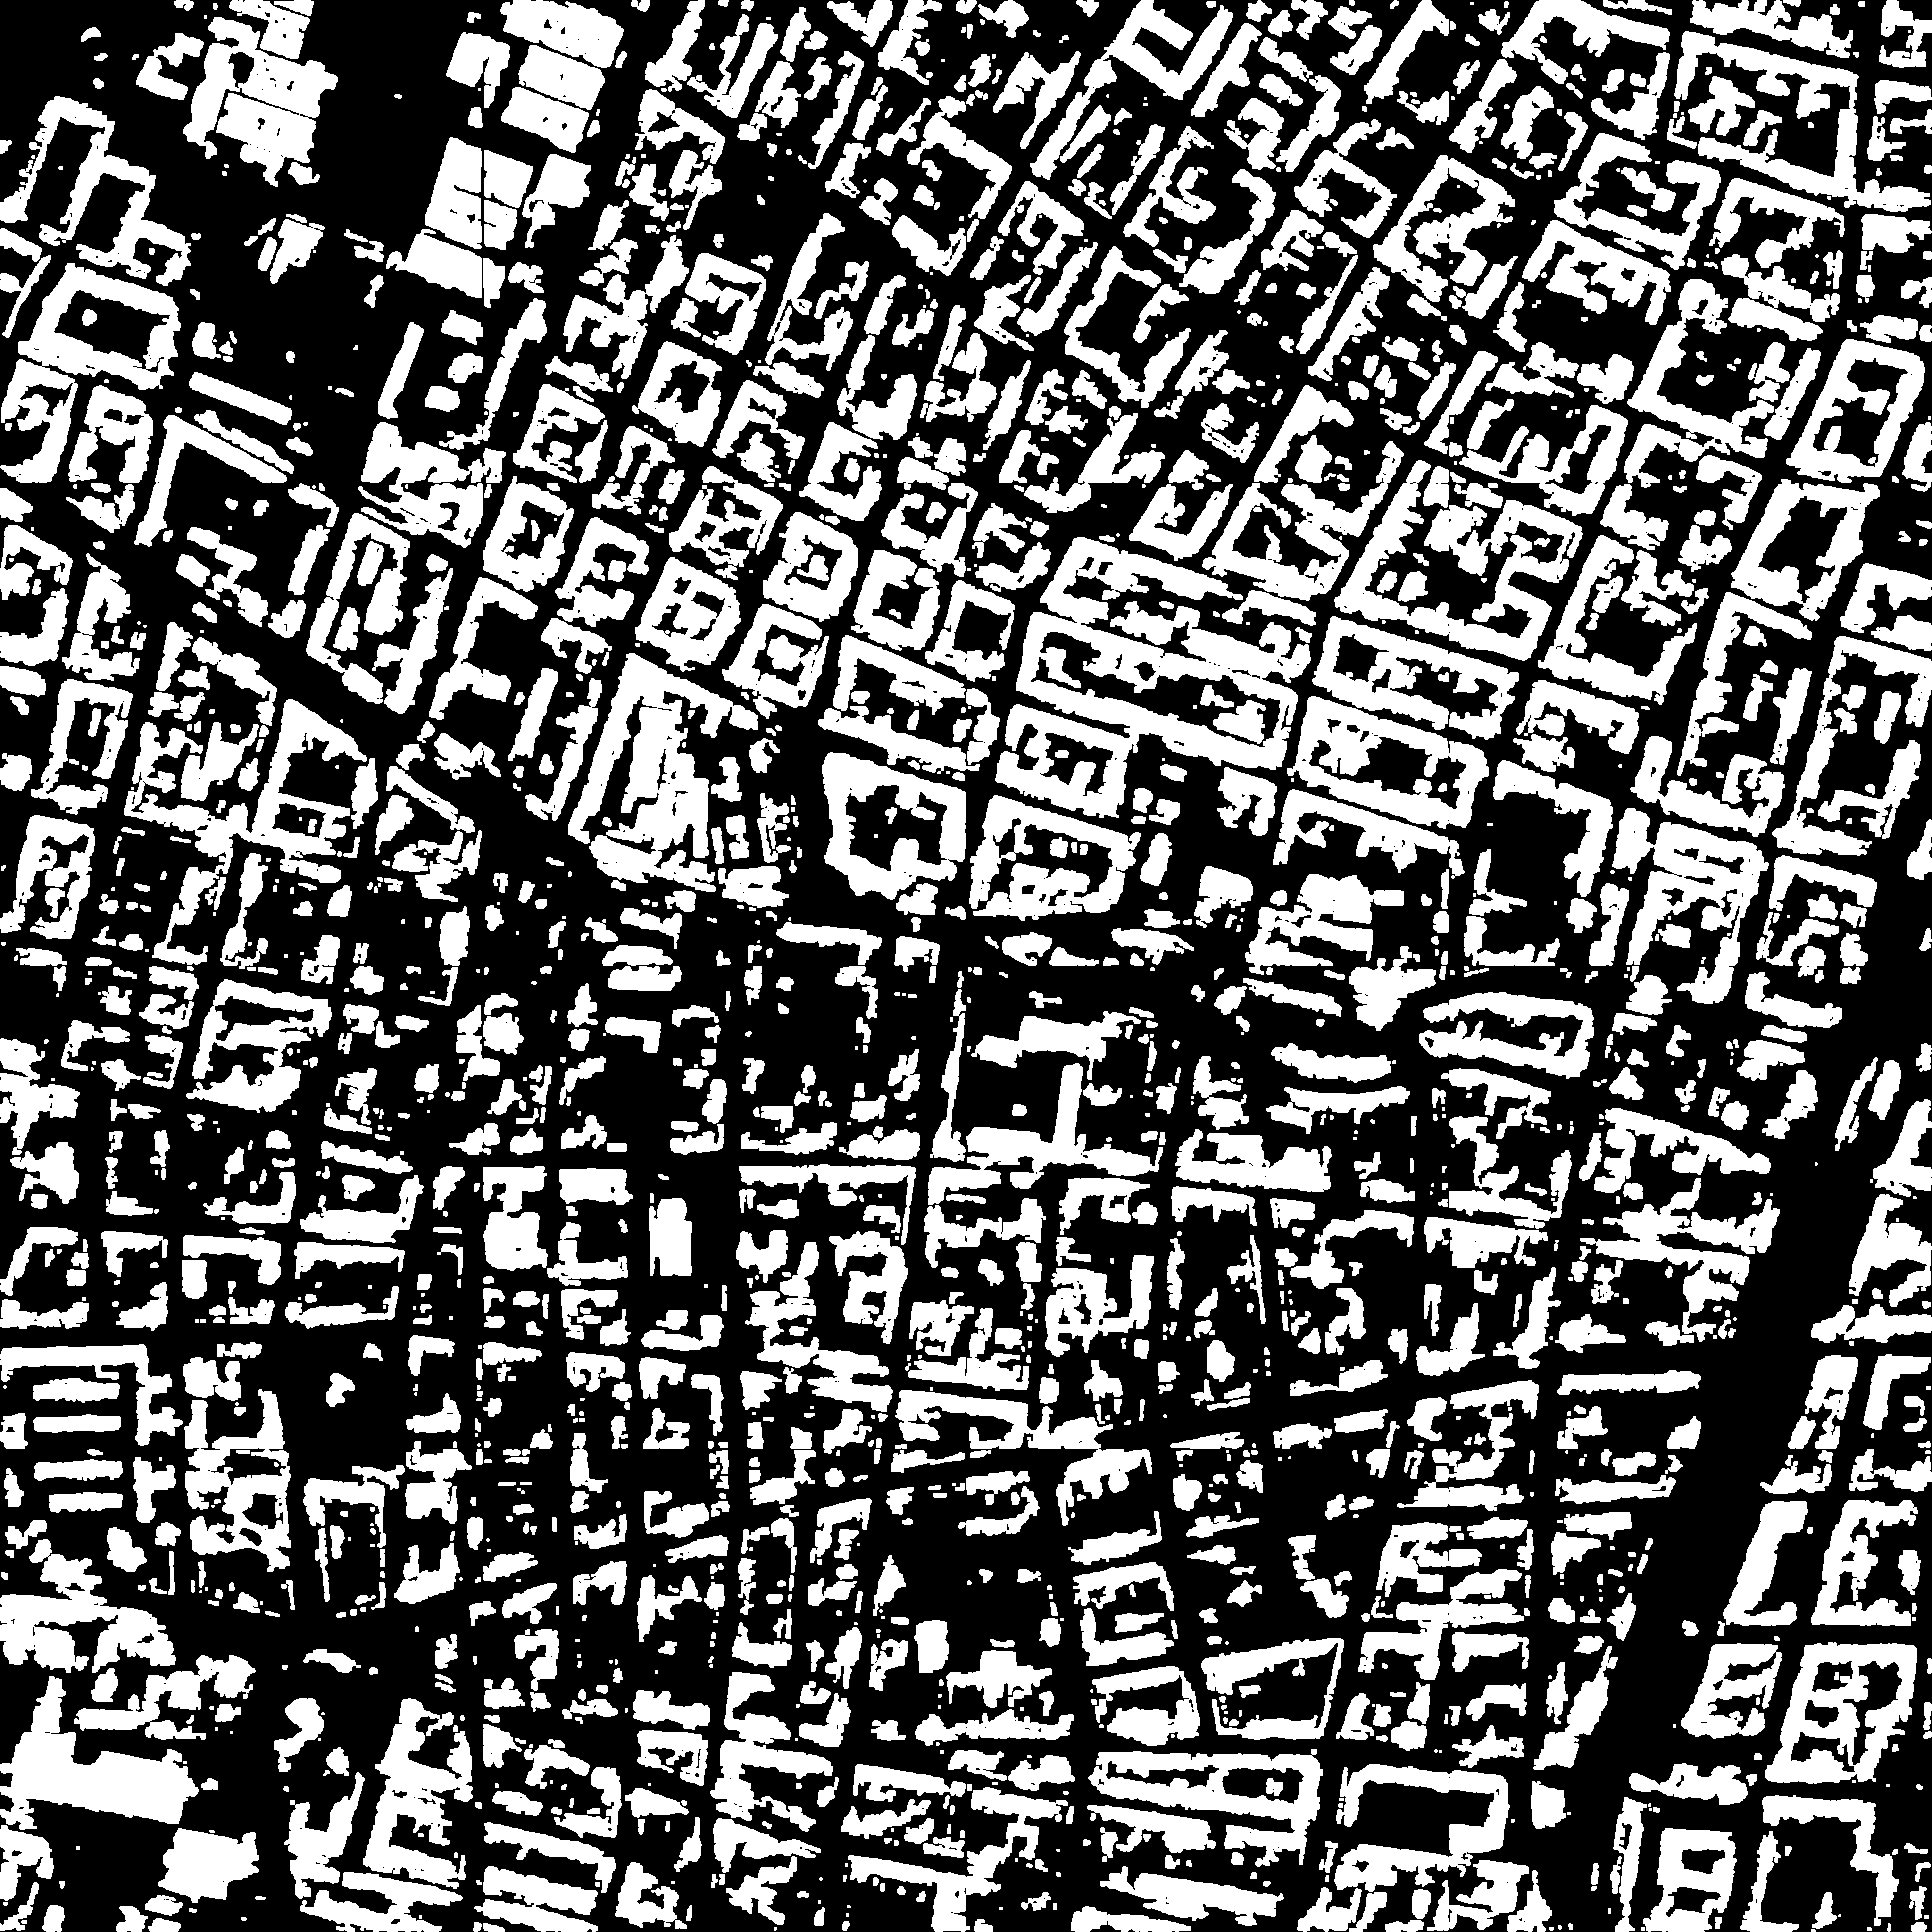
\includegraphics[width=1\linewidth]{Figures/结果/vienna8_平衡_中值滤波.png}
        \caption{维也纳—类别平衡交叉熵}
        \label{Fig:test_image_2_cbce}
    \end{minipage}
    
\end{figure}
维也纳地区图像,使用交叉熵作为损失函数训练出来的卷积神经网络的正确率为0.84,使用类别平衡交叉熵作为损失函数训练出来的卷积神经网络的正确率为0.83。

维也纳地区街道呈“口”字型。使用类别平衡交叉熵作为损失函数的网络建筑更加完整,部分街道被两侧的房屋侵蚀。使用交叉熵作为损失函数的网络街道纹理没有使用类别平衡交叉熵完整,但街道错认情况较类别平衡交叉熵轻微。


图\ref{Fig:test_image_2}是奥斯汀地区的遥感图像;图\ref{Fig:test_image_2_gt}是该地区遥感图像的ground-truth。
\begin{figure}[htbp]
    
    \centering
    \begin{minipage}[t]{0.49\linewidth}
        \centering
        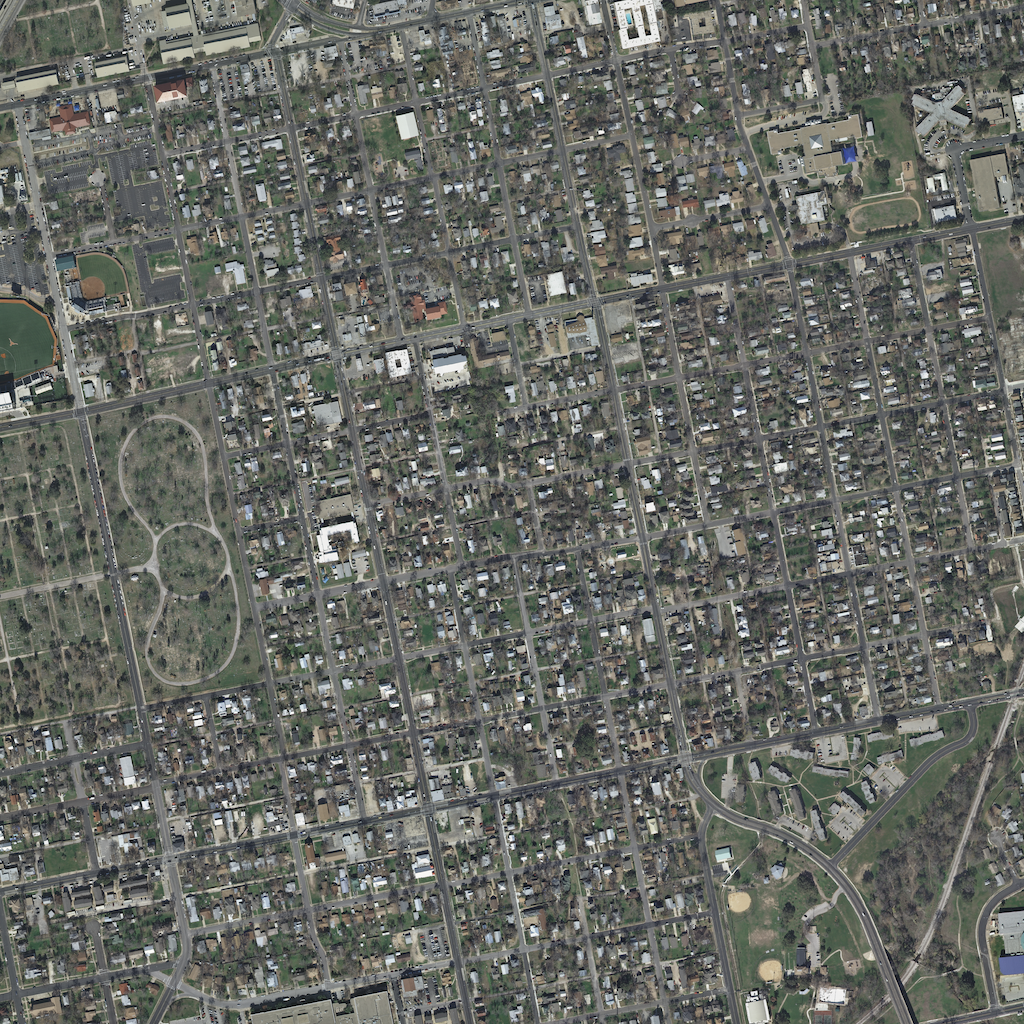
\includegraphics[width=1\linewidth]{Figures/结果/austin29.png}
        \caption{奥斯汀}
        \label{Fig:test_image_2}
    \end{minipage}
    \begin{minipage}[t]{0.49\linewidth}
        \centering
        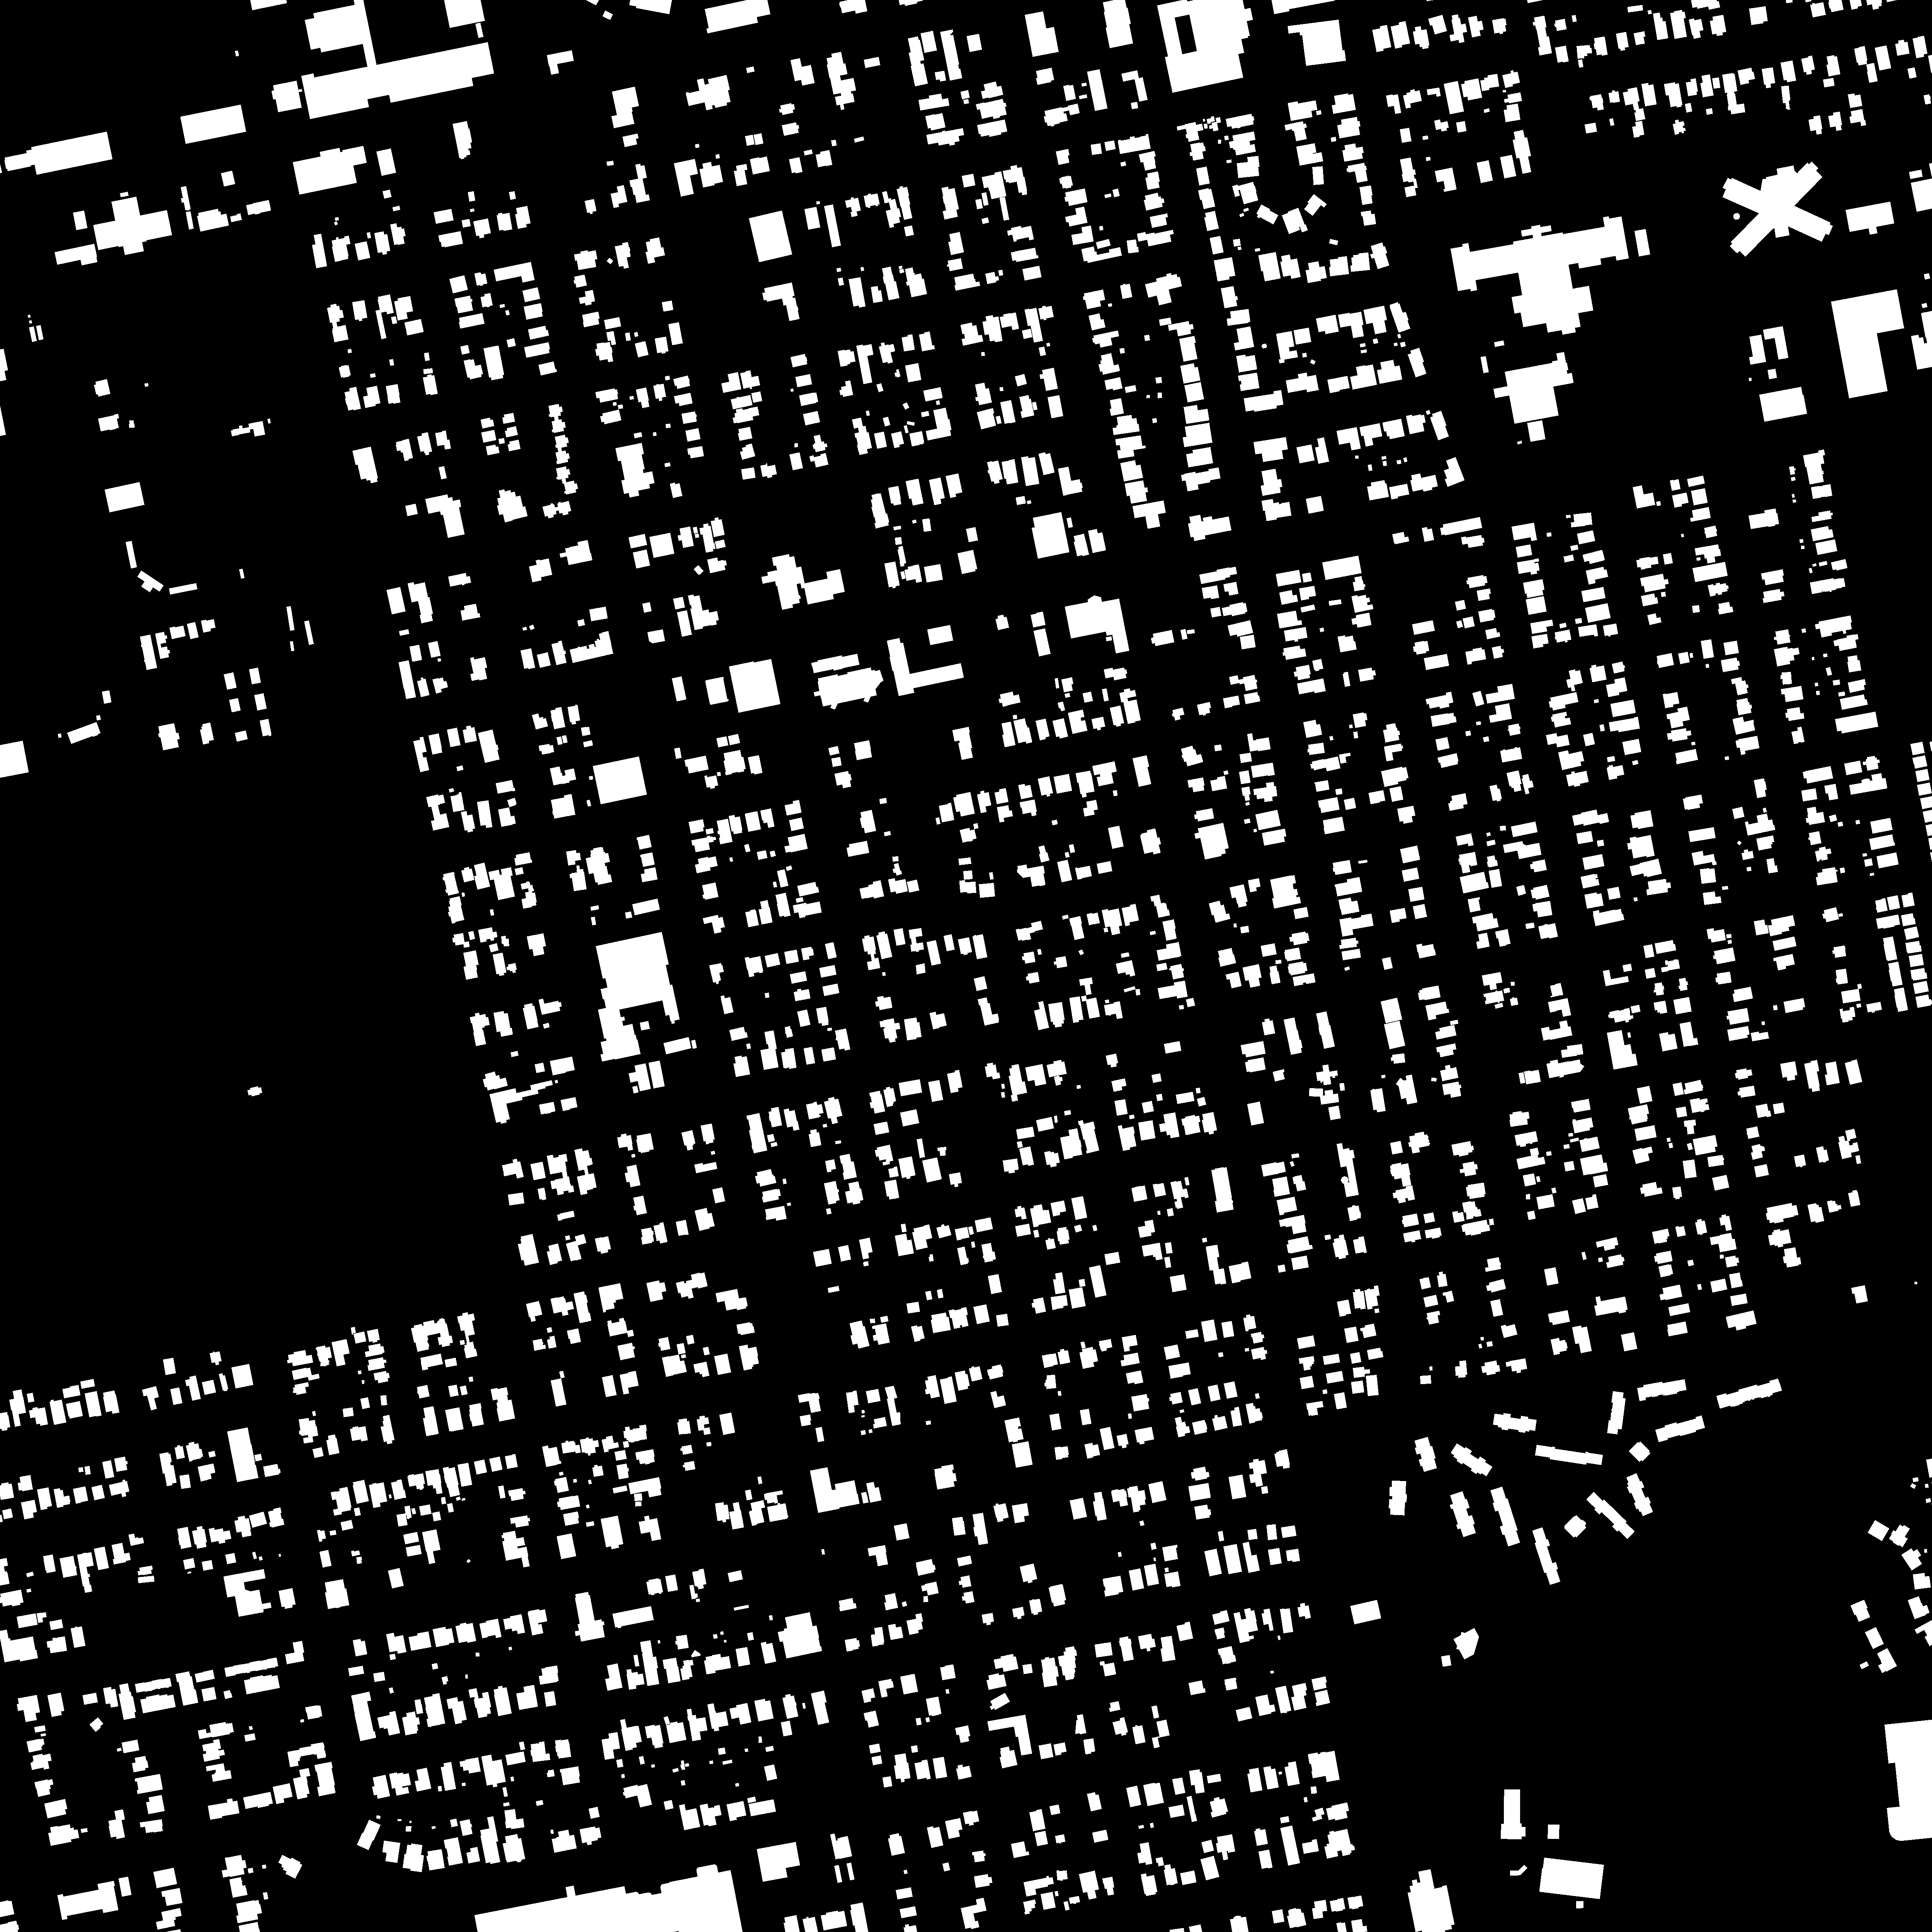
\includegraphics[width=1\linewidth]{Figures/结果/austin29_gt.png}
        \caption{奥斯汀ground-truth}
        \label{Fig:test_image_2_gt}
    \end{minipage}
    
\end{figure}

图\ref{Fig:test_image_2_ce}是使用交叉熵作为损失函数的奥斯汀地区的预测结果;图\ref{Fig:test_image_2_cbce}是使用类别平衡交叉熵作为损失函数的奥斯汀地区的预测结果。
\begin{figure}[htbp]
    
    \centering
    \begin{minipage}[t]{0.49\linewidth}
        \centering
        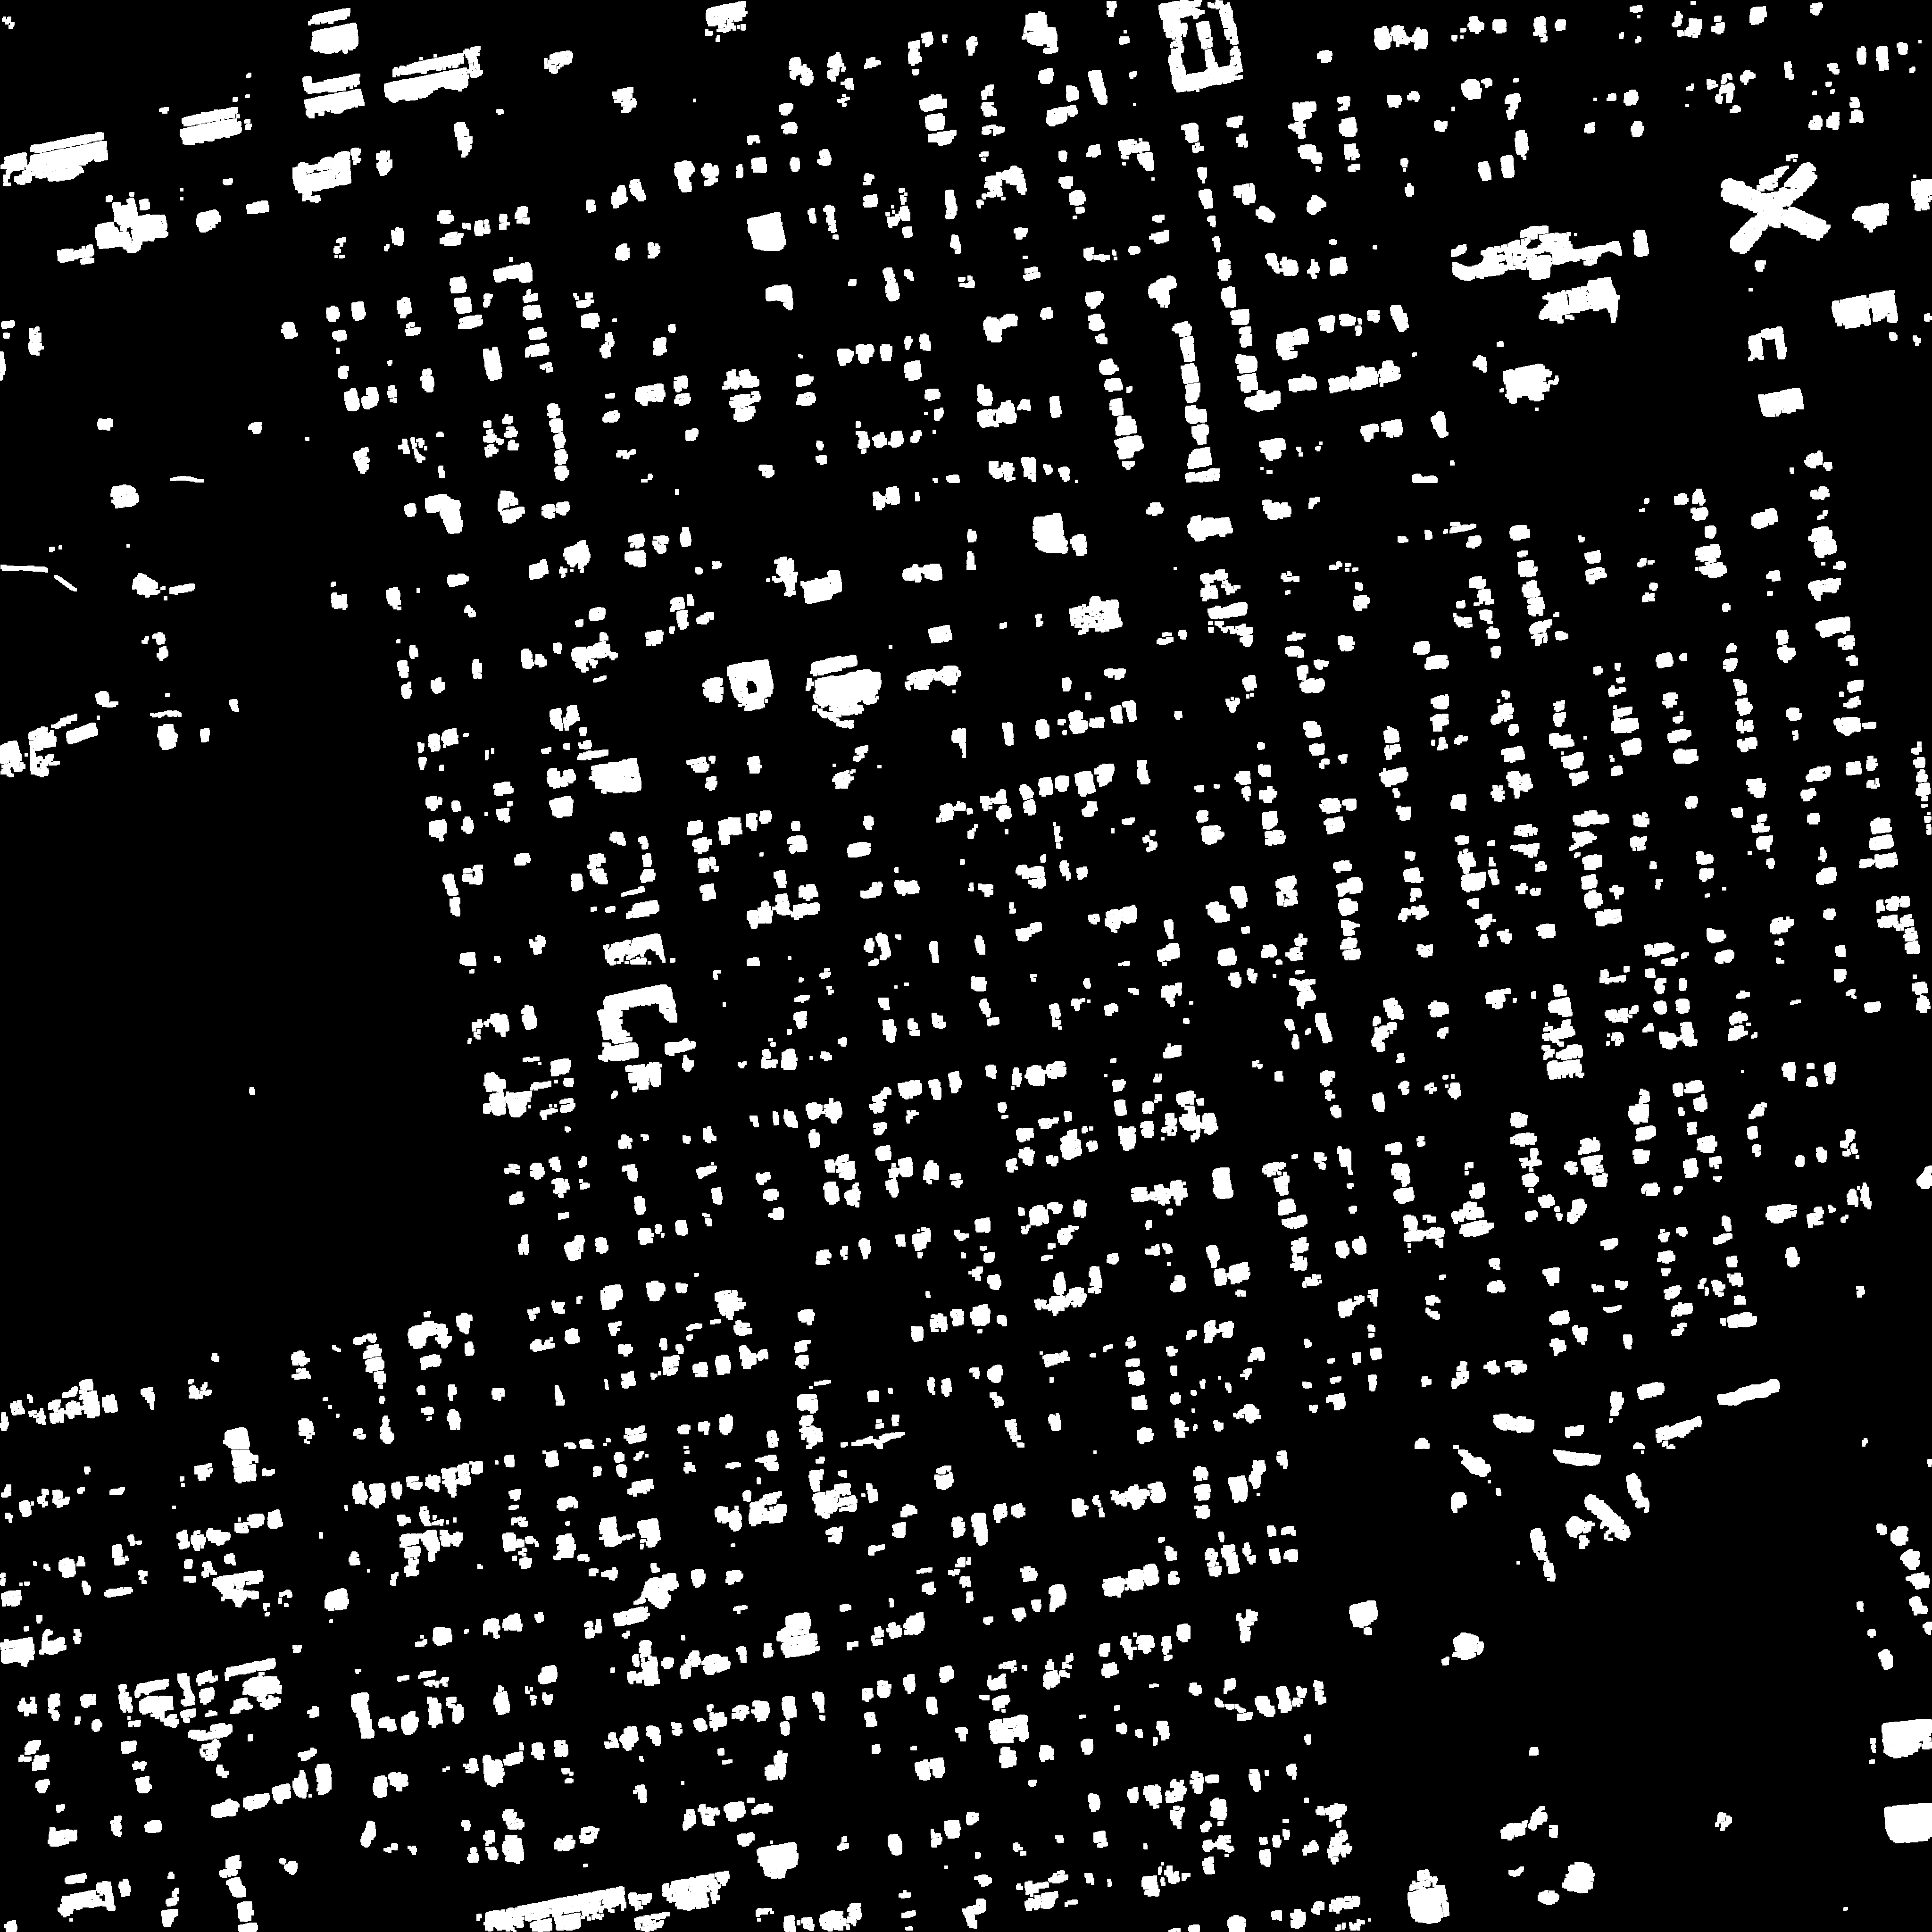
\includegraphics[width=1\linewidth]{Figures/结果/austin29_交叉熵.png}
        \caption{奥斯汀—交叉熵}
        \label{Fig:test_image_2_ce}
    \end{minipage}
    \begin{minipage}[t]{0.49\linewidth}
        \centering
        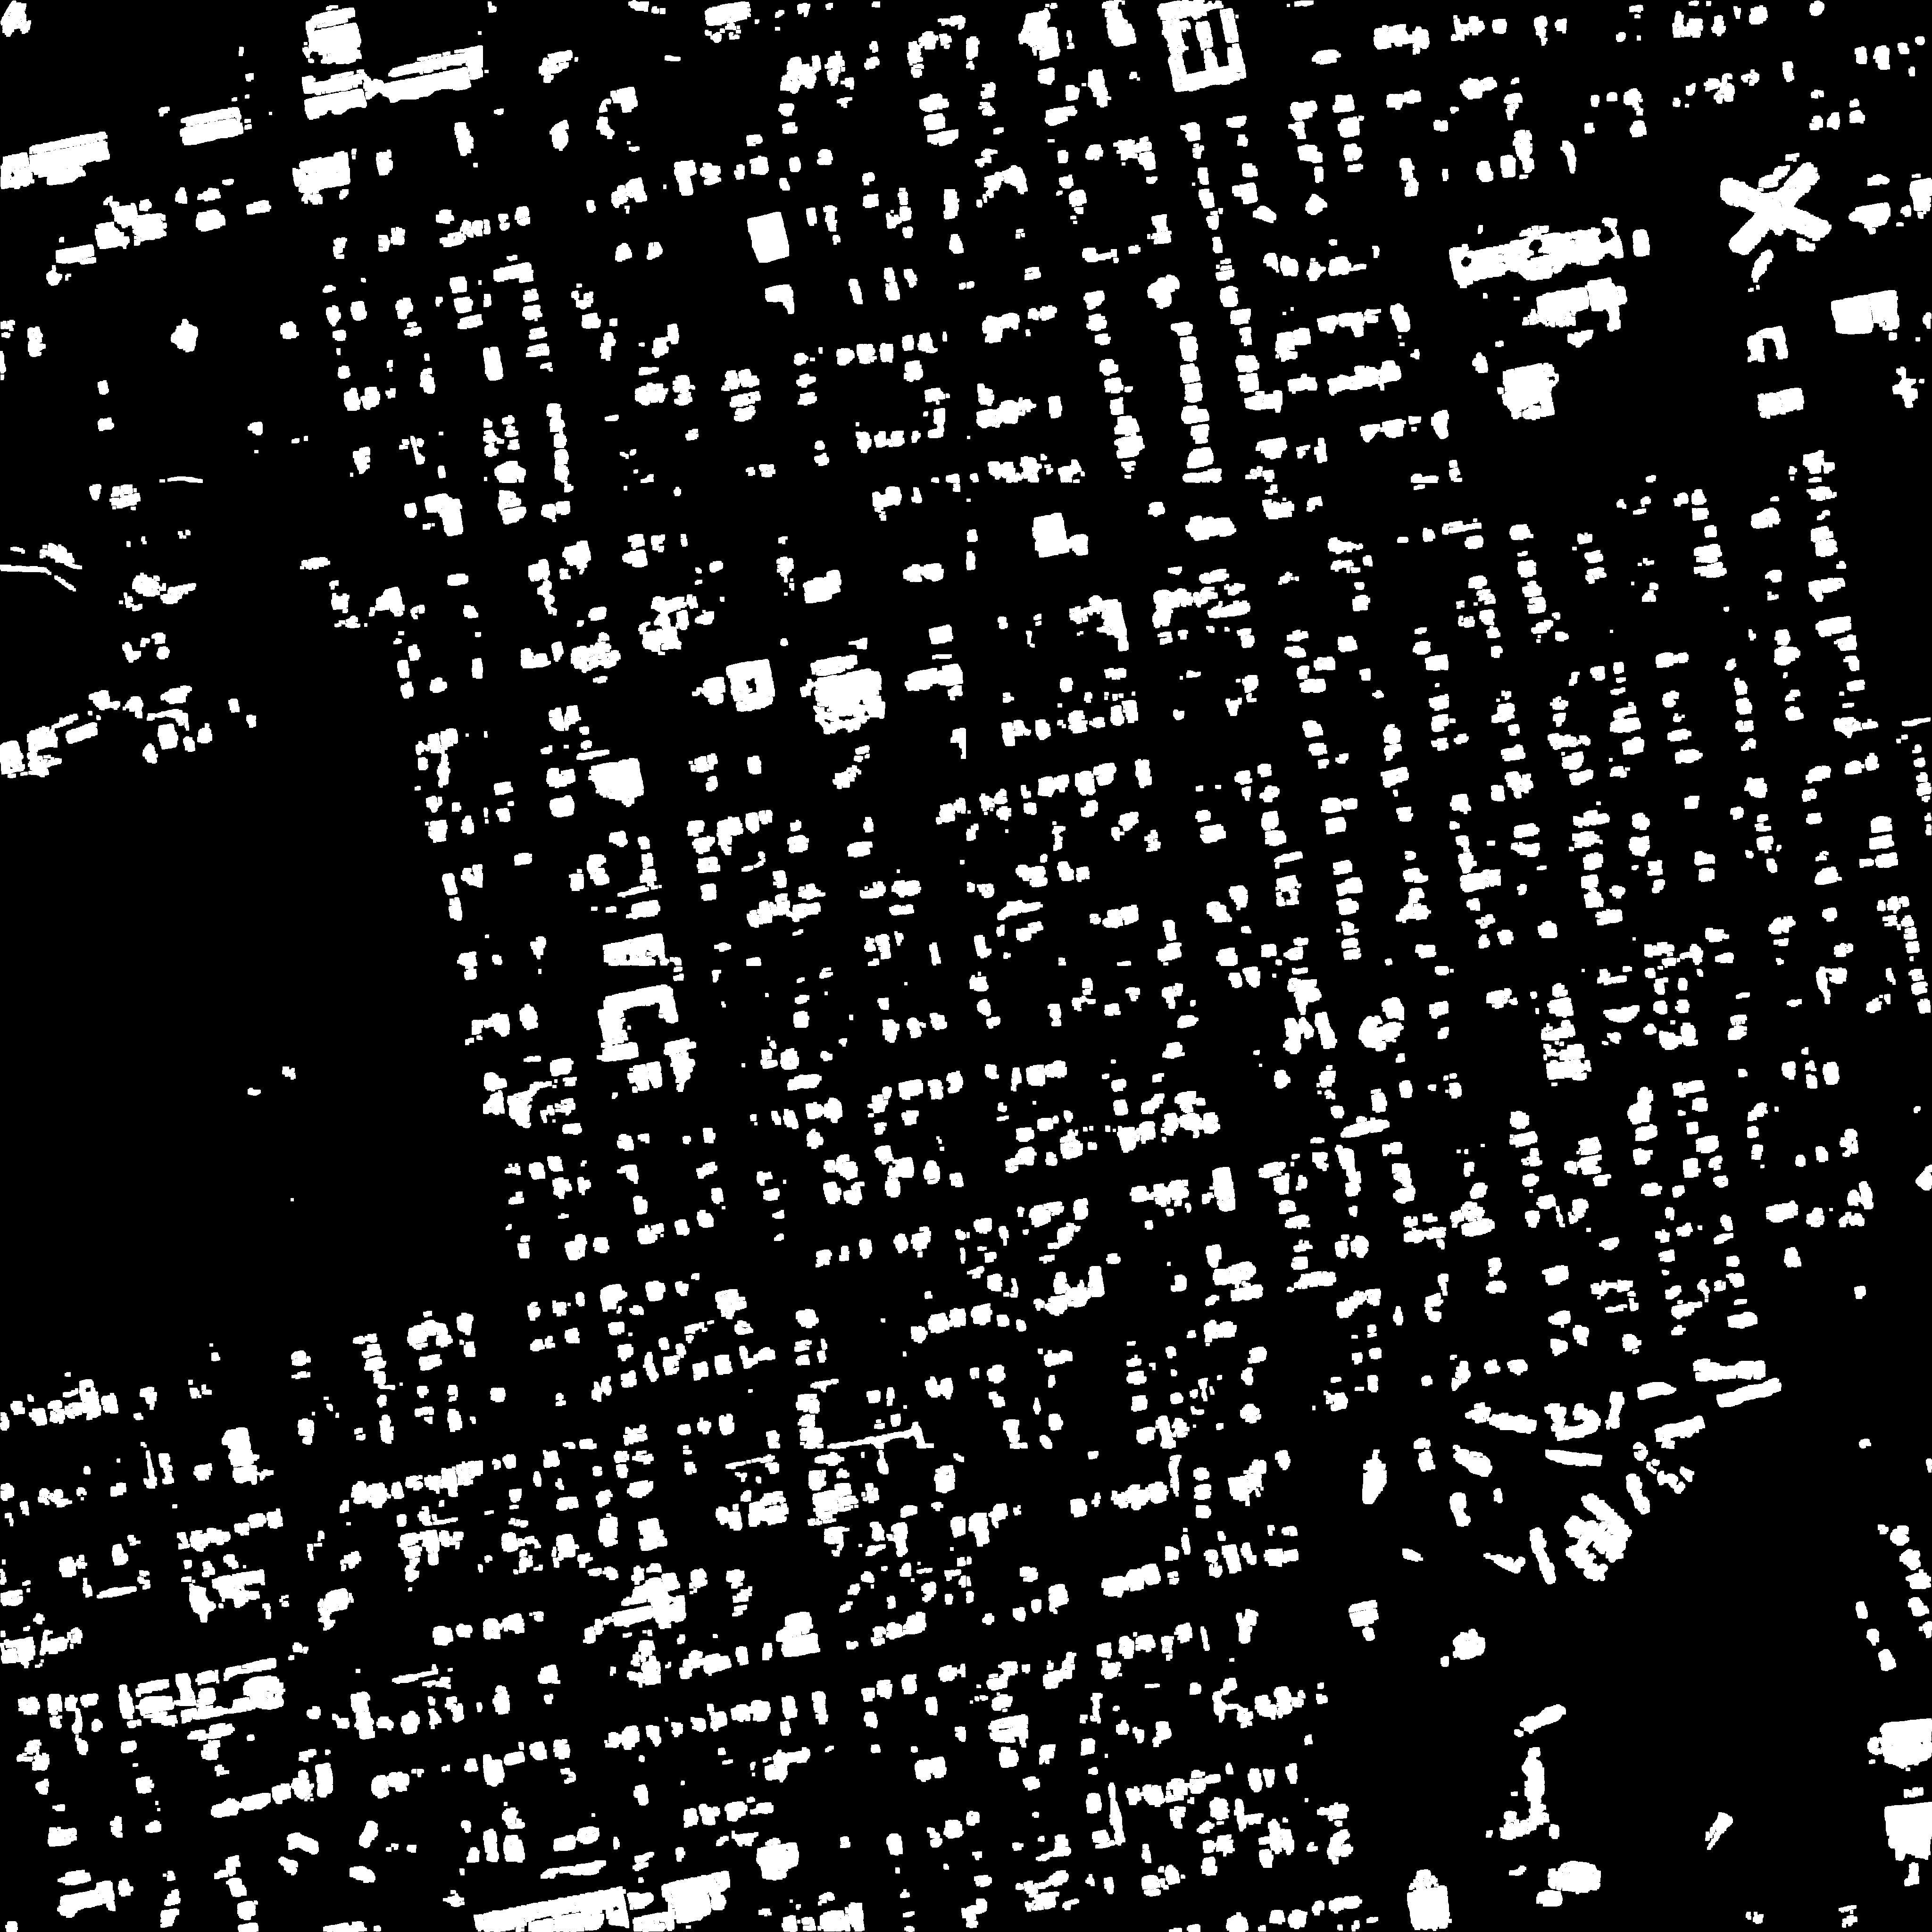
\includegraphics[width=1\linewidth]{Figures/结果/austin29_平衡.png}
        \caption{奥斯汀—类别平衡交叉熵}
        \label{Fig:test_image_2_cbce}
    \end{minipage}
    
\end{figure}


奥斯汀地区图像,使用交叉熵作为损失函数训练出来的卷积神经网络的正确率为0.81,使用类别平衡交叉熵作为损失函数训练出来的卷积神经网络的正确率为0.80。

奥斯汀地区房屋呈点状分布。使用类别平衡交叉熵作为损失函数的网络大型建筑的识别较交叉熵完整,且房屋单个房屋的形状更加规整。使用交叉熵作为损失函数结果在大型建筑的识别上存在空洞。单个中小型建筑的外围也没有类别平衡交叉熵规则。

